\section{Tensors as Multilinear Maps}

  There are multiple ways to construct tensor product spaces. Note that all the constructions are equivalent and will lead to the exact same properties of tensors. The first method defines tensors outright as multilinear maps, without the need for a basis. 

\subsection{Tensor Product of Two Spaces}

  \begin{definition}
  The tensor product of two vector spaces $V$ and $W$ is a vector space, denoted $V \otimes W$, created by the bilinear map 
  \[\otimes: V \times W \longrightarrow V \otimes W, \; (x, y) \mapsto x \otimes y\]
  That is, 
  \[V \otimes W \equiv \{ x \otimes y \; | \; x \in V, y \in W\} \]
  where the elements of $V \otimes W$ are called \textbf{tensors}. Note that since we have defined the operation $\otimes$ to be bilinear, it satisfies the properties
  \begin{enumerate}
      \item $(u_1 + u_2) \otimes v = u_1 \otimes v + u_2 \otimes v$
      \item $v \otimes (u_1 + u_2) = v \otimes u_1 + v \otimes u_2$
      \item $(\lambda u) \otimes v = u \otimes (\lambda v) = \lambda (u \otimes v)$ 
  \end{enumerate}
  Moreover, each tensor $x \otimes y$ is itself a bilinear operator
  \[x \otimes y: V^* \otimes W^* \longrightarrow \mathbb{F}\]
  \end{definition}

  Using these properties we will deduce further qualities of tensor product spaces. First, given a basis $\{e_i\}$ of $n$-dimensional space $V$ and $\{f_j\}$ of $m$-dimensional space $W$, we can construct a basis 
  \[\{e_i \otimes f_j \; | \; 1 \leq i \leq n, 1 \leq j \leq m\}\]
  of $V \otimes W$ using only the bilinearity properties of $\otimes$. 

  \begin{example}
  Let $V^*$ be a 4-dimensional vector space with basis $\{ e^0, e^1, e^2, e^3\}$. Then the basis of $V^* \otimes V^*$ is
  \begin{align*} 
  \{e^0 \otimes e^0, \; e^0 \otimes e^1, \;e^0 \otimes e^1, \;e^0 \otimes e^1, \\
  e^1 \otimes e^0,\; e^1 \otimes e^1,\; e^1 \otimes e^2,\; e^1 \otimes e^3, \\
  e^2 \otimes e^0,\; e^2 \otimes e^1,\; e^2 \otimes e^2,\; e^2 \otimes e^3, \\
  e^3 \otimes e^0,\; e^3 \otimes e^1,\; e^3 \otimes e^2,\; e^3 \otimes e^3\}
  \end{align*}
  \end{example}

  That is, every tensor can be expressed as a linear combination of these vectors, which implies
  \[\dim{V \otimes W} = (\dim{V}) (\dim{W})\]
  By equality of dimensionality and bilinearity, it is obvious that
  \[V \otimes W \simeq \text{Hom}(V \times W, \mathbb{F})\]
  In fact, they are naturally isomorphic. 

  Notice that we still haven't actually defined how to "calculate" using the operator $x \otimes y$. It turns out that defining a tensor product is unique up to isomorphism. That is, if $(V \otimes W, \otimes_1)$ and $(V \otimes W, \otimes_2)$ are two tensor product spaces sufficing bilinearity, then $V \otimes_1 W \simeq V \otimes_2 W$. This result is formally stated in the proposition below. 

  \begin{proposition}[Universal Property of 2-tensors]
  With this constructed basis, we can claim that for every map $\varphi: V \times W \longrightarrow \mathbb{F}$, there exists a unique linear map $\psi: V \otimes W \longrightarrow \mathbb{F}$ such that 
  \[\varphi (x, y) = \psi (x \otimes y) \; \forall x \in V, y \in W\]
  \end{proposition}
  \begin{proof}
  Since $\{e_i \otimes f_j\}$ is a basis for $V \otimes W$, we know that every element $z \in V \otimes W$ decomposes uniquely into 
  \[z = \sum_{i, j} z_{i j} e_i \otimes f_j, \; z_{i j} \in \mathbb{F}\]
  Thus, by linearity it suffices to define these maps for the basis vectors. This linear map is determined as 
  \[\psi (e_i \otimes f_j) = \varphi (e_i, f_j)\]
  \end{proof}
  Denoting the map that is defined by taking all $e_i \otimes f_j \mapsto (e_i, f_j)$ as $S$, we can see that $S$ is clearly an isomorphism defined such that the diagram below commutes. 
  \[\begin{tikzcd}
      V \otimes W \arrow{r}{\psi} \arrow{d}{S} & \mathbb{F} \\
      V \times W \arrow{ru}{\varphi}
  \end{tikzcd}\]
  That is, the unique isomorphism $S$ exists that determines $\psi$ such that 
  \[\psi = \varphi \circ S \] 
  which means that all definitions of $\otimes$ are equivalent under $S$. Note further that $S$ determines the isomorphism 
  \[(V \otimes W)^* \equiv \text{Hom}(V \otimes W, \mathbb{F}) \simeq \text{Hom}(V \times W, \mathbb{F})\]
  Therefore, it does not matter how we choose to concretely define the operator $x \otimes y$ for computations. However, it is customary to define it as
  \[(x \otimes y) (\alpha, \beta) = \alpha (x) \cdot \beta (y), \; \alpha \in V^*, \beta \in W^*\]
  Given $x \otimes y \in V \otimes W$, we can also choose to input elements "partially." That is, if we only input one vector $\alpha \in V^*$ into $x \otimes y$, we get
  \[(x \otimes y) (\alpha, \cdot) = \alpha(x) y (\cdot) = \alpha (x) y \in W\]
  meaning that the isomorphisms below are all canonical
  \[V \otimes W \simeq \text{Hom}(V \times W, \mathbb{F}) \simeq \text{Hom}(V^*, W)\]
  This means that
  \[V^* \otimes W \simeq \text{Hom}(V, W)\]
  That is, an element $\alpha \otimes y \in V^* \otimes W$ is a linear map from $V$ to $W$! We will focus a bit more on elements of $V^* \otimes W$. Given the previous bases $e_i$ and $f_j$ for $V$ and $W$, let $\{\epsilon_i\}$ be the dual basis for $V^*$. Then, the tensor $\alpha \otimes w \in V^* \otimes W$ can be represented as 
  \begin{align*}
      \alpha \otimes w & \equiv \bigg(\sum_i \alpha_i \epsilon_i \bigg) \otimes \bigg( \sum_j w_j f_j \bigg) \\
      & = \sum_{i, j} \alpha_i w_j \, \epsilon_i \otimes f_j = \sum_{i, j} A_{i j} \, \epsilon_i \otimes f_j
  \end{align*}
  In fact, the $A_{i j}$ are precisely the $i j$th components of the matrix representation of linear operator $\alpha \otimes y$ with respect to basis $\{\epsilon_i\}$ and $\{f_j\}$. Indeed,
  \begin{align*}
      (\alpha \otimes y)(e_j) & = \bigg( \sum_{i, j} e_i \otimes f_j \bigg) e_j \\
      & = \sum_{i, j} A_{i j} e_i \cdot \delta^j_j = \sum_{i} A_{i j} e_i
  \end{align*}
  which is consistent with the column space interpretation of matrix multiplication discussed in the beginning of Chapter 4. The realization of this tensor product between a covector and a vector is realized as an \textbf{outer product}. 

  \begin{definition}
  Given vector spaces $U, V$ with defined bases in each of them, the \textbf{outer product} of two vectors $u \in U$ and $v \in V$ is defined
  \[u \otimes v \equiv u v^T \equiv \begin{pmatrix}
  u_1 \\ u_2 \\ ... \\ u_m
  \end{pmatrix} \otimes \begin{pmatrix}
  v_1 & ... & v_n
  \end{pmatrix} = \begin{pmatrix}
  u_1 v_1 & ... & u_1 v_n \\
  u_2 v_1 & ... & u_2 v_n \\
  ... & ... & ... \\
  u_m v_1 & ... & u_m v_n 
  \end{pmatrix}\]
  Note that the $\otimes$ symbol in here represents the outer product, not the tensor product. Note that the tensor rank of the outer product of two vectors is $(2,0)$. 
  \end{definition}

  Abstractly speaking, the outer product of $u \in U$ and $v \in V$ is the element $u \otimes v \in U \otimes V$, which is a rank-(2,0) tensor, not a rank-(1,1) tensor! Just because it "looks" like a matrix, $u \otimes v$ should not be interpreted as a linear map. Such a $m \times n$ matrix could really be the realization of either a (2,0) tensor, (1,1) tensor, or a (0,2) tensor. 

  However, if $U$ is an inner product space, then it is possible to define $u \times v$ as a linear map from $U \longrightarrow W$. The structure of the inner product on $U$ allows us to define the canonical isomorphism $\phi$ between $U$ and $U^*$. Then, we can define the canonical injections $i: U \longrightarrow U \otimes V$ and $j: U^* \longrightarrow U^* \otimes V$ to get the commutative diagram 

  \[\begin{tikzcd}
      U \otimes V \arrow{r}{\gamma} & U^* \otimes V \\
      U \arrow{u}{i} \arrow{r}{\phi} & U^* \arrow{u}{j}
  \end{tikzcd}\]
  Given that 
  \[\phi(u) \equiv l \text{ such that } (u, x) = l(x) \forall x \in U\]
  we can define the mapping $\gamma: j \phi i^{-1}$ such that 
  \[\gamma (u \otimes v) \equiv \phi(u) \otimes v \equiv l \otimes v \in U^* \otimes V\]
  which is ultimately a linear mapping from $U \longrightarrow V$ since
  \[l \otimes v (u_0, \cdot) \equiv l(u_0) v(\cdot)\]
  with $l(u_0) \in \mathbb{F}$ and $v(\cdot)$ a vector. This proves the following theorem. 

  \begin{proposition}
  The matrix rank of the outer product of any 2 vectors is $1$. 
  \end{proposition}
  \begin{proof}
  Trivial.
  \end{proof}

  We can extrapolate and see that for higher order tensor products, we would get an $n$-dimensional array of scalars. A matrix is a $2$-dimensional array of numbers since it is the tensor product of two vectors. 

  \begin{definition}
  Given vector spaces $U, V$ with defined bases in each of them, the \textbf{Kronecker product} of two vectors $u \in U$ and $v \in V$ is defined
  \[u \otimes_{Kron} v \equiv \begin{pmatrix}
  u_1 \\ u_2 \\ ... \\ u_m
  \end{pmatrix} \otimes \begin{pmatrix}
  v_1 & ... & v_n
  \end{pmatrix} = \begin{pmatrix}
  u_1 v_1 \\ u_1 v_2 \\ ... \\ u_m v_{n-1} \\ u_m v_n 
  \end{pmatrix}\]
  \end{definition}

  Clearly, the outer product and Kronecker product are closely related, and we can interpret the Kronecker product as a form of "vectorization" or "flattening out" of the outer product. 

\subsection{Higher Order Tensor Product Spaces}

  Since $U \otimes W$ is a vector space itself, we can multiply it further to create higher order tensor product spaces. 
  \[U \otimes W \otimes U \otimes ...\]
  Note that by construction, the operation of tensor product on vector spaces is commutative and associative in the sense that 
  \[V \otimes W \simeq W \otimes V\]
  and 
  \[(U \otimes V) \otimes W \simeq U \otimes (V \otimes W) \simeq U \otimes V \otimes W \]
  which allows us to write tensor products of any finite number of vector spaces $V_1, V_2, ..., V_n$ without parantheses. By induction, we can keep constructing higher order tensor products as such 
  \[V_1 \otimes V_2 \rightarrow (V_1 \otimes V_2) \otimes V_3 \rightarrow \big((V_1 \otimes V_2) \otimes V_3 \big) \otimes V_4 \rightarrow ...\]
  to get the tensor product space
  \[\bigotimes_{i=1}^{n} V_{i} \equiv V_1 \otimes V_2 \otimes ... \otimes V_n\]
  with tensors in the form 
  \[ \bigotimes_{i=1}^{n} v_{i} \equiv v_{1} \otimes v_{2} \otimes v_{3} \otimes ... \otimes v_{n}; \; v_{i} \in V_{i}\]
  defined as the following multilinear map 
  \[ \bigotimes_{i=1}^{n} v_{i}: \prod_{i=1}^{n} V_{i}^{*} \longrightarrow \mathbb{F}, \;\;\; \bigg( \bigotimes_{i=1}^{n} v_{i} \bigg) \big( l_{1}, l_{2}, ..., l_{n} \big) \equiv \prod_{i=1}^{n} v_{i}(l_{i}), \; l_i \in V_i^* \]
  This map can then be used to easily see the following statement
  \[\bigotimes_{i=1}^n V_i \simeq \text{Hom}\Big( \prod_{i=1}^n V_i^*, \mathbb{F} \Big)\]
  Similarly to the section about the tensor product of two spaces, we can "partially" fill in the inputs of a general tensor $v_1 \otimes v_2 \otimes ... \otimes v_n$ to interpret them as multilinear operators that can take in $k$ vectors and output $n-k$ vectors. That is, tensors (written as $\tau$ below) are multilinar maps from a cartesian product of vector spaces to a tensor product of vector spaces. 
  \[\tau: V_1 \times ... \times V_n \longrightarrow W_1 \otimes ... \otimes W_m \]
  For example, 
  \[\text{Hom}\Big( \prod_{i=1}^n V_i^*, \mathbb{F} \Big) \simeq 
  \text{Hom}\Big( \prod_{i=2}^n V_i^*, V_1 \Big) \simeq 
  \text{Hom}\Big( \prod_{i=3}^n V_i^*, V_1 \otimes V_2 \Big) \simeq ... \]
  Furthermore, we can generalize the universal property of two tensors to the following proposition, which is also called the \textbf{fundamental principle of tensor algebra}. 

  \begin{proposition}[Universal Property]
  Given a linear mapping $\varphi: V_1 \times ... \times V_n \longrightarrow \mathbb{F}$, there exists a unique linear map $\psi: V_1 \otimes ... \otimes V_n \longrightarrow \mathbb{F}$. That is, 
  \[\text{Hom}\Big( \bigotimes_{i=1}^n V_i, \mathbb{F} \Big) \equiv \bigg( \bigotimes_{i=1}^n V_i \bigg)^* \simeq \text{Hom}\Big(\prod_{i=1}^n V_i, \mathbb{F}\Big)\]
  \end{proposition}

  \begin{definition}
  Given that 
  \[ \{ e_{i_{j}}\}_{i_{j}=1}^{k_{j}} \text{ of } V_{j},\; j = 1, 2, ..., n\]
  are $n$ sets of bases for each $V_{j}$, 
  \[ \{ \bigotimes_{j=1}^{n} e_{i_{j}} \}_{i_{1}, ..., i_{n}} \text{ is a basis of } \bigotimes_{j=1}^{n} V_{j}\]
  \end{definition}

  \begin{proposition}
  Given vector spaces $V_1, V_2, ..., V_n$, 
  \[ \dim \bigotimes_{i=1}^{n} V_i = \prod_{i=1}^{n} \dim V_{i}\]
  \end{proposition}
  \begin{proof}
  This follows naturally from the construction of the basis.
  \end{proof}

  We move on to talk about something quite enlightening: the tensor product of linear operators, which are themselves tensors. 

  \begin{definition}
  Given linear operators $A \in $ End$(V)$, $B \in $ End$(W)$, we can construct the linear operator 
  \[A \otimes B \in \text{End}(V \otimes W)\] 
  such that 
  \[(A \otimes B) (x \otimes y) \equiv A x \otimes B y \in V \otimes W\]
  Notice that since $A, B$ are linear operators, they are tensors. More specifically, $A \equiv \alpha \otimes u$ and $B \equiv \beta \otimes v$, so
  \begin{align*}
      (A \otimes B) (x \otimes y) & \equiv A x \otimes B y \\
      & = (\alpha \otimes u) x \otimes (\beta \otimes v) y \\
      & = \alpha (x) \beta (y) \, u \otimes v \\
      & = \big((\alpha \otimes \beta)(x \otimes y)\big) (u \otimes v)(\cdot, \cdot) \\
      & = \big((\alpha \otimes \beta) \otimes (u \otimes v)\big) \big((x \otimes y), (\cdot \otimes \cdot)\big) \\
      & = \big((\alpha \otimes \beta) \otimes (u \otimes v)\big)(x \otimes y) 
  \end{align*}
  $\implies A \otimes B \equiv \alpha \otimes \beta \otimes u \otimes v$. 
  \end{definition}
  We will work through an example that gives the matrix representation of the tensor product of linear mappings. For simplicity, let us work with the example when 
  \[A = \begin{pmatrix}
  a_{11} & a_{12} \\ a_{21} & a_{22}
  \end{pmatrix}, \; B = \begin{pmatrix}
  b_{11} & b_{12} \\ b_{21} & b_{22}
  \end{pmatrix}\]
  Given that $U$ has basis $\{u_1, u_2\}$ and $V$ has basis $\{v_1, v_2\}$, $U \otimes V$ will have basis 
  \[\{u_1 \otimes v_1, u_1 \otimes v_2, u_2 \otimes v_1, u_2 \otimes v_2\}\]
  We then define the induced linear mapping $A\otimes B: U \otimes V \longrightarrow U \otimes V$ by defining it on its basis vectors. Note that the linear mapping $(A \otimes B)(u\otimes v)$ must be an element of $U \otimes V$, implying that it is defined
  \[(A \otimes B)(u\otimes v) \equiv Au \otimes Bv\]
  This is called the \textbf{tensor product} of operators $A$ and $B$.
  So, the tensor product of matrices $A$ and $B$ can be calculated
  \begin{align*}
      (A \otimes B) (u_1 \otimes v_1) &= (a_{11} u_1 + a_{21} u_2) \otimes (b_{11} v_1 + b_{21} v_2) \\
      & = a_{11} b_{11} (u_1 \otimes v_1) + a_{11} b_{21} (u_1 \otimes v_2) \\
      & + a_{21} b_{11} (u_2 \otimes v_1) + a_{21} b_{21} (u_2 \otimes v_2) \\
      ... & = ... \\
      (A \otimes B) (u_2 \otimes v_2) & = (a_{12} u_1 + a_{22} u_2) \otimes (b_{12} v_1 + b_{22} v_2) \\
      & = a_{12} b_{12} (u_1 \otimes v_1) + a_{12} b_{22} (u_1 \otimes v_2) \\
      & + a_{22} b_{12} (u_2 \otimes v_1) + a_{22} b_{22} (u_2 \otimes v_2) 
  \end{align*}
  In matrix form, this results in the $4\times 4$ matrix (also in block form)
  \[A \otimes B \equiv \begin{pmatrix}
  a_{11} b_{11} & a_{11} b_{12} & a_{12} b_{11} & a_{12} b_{12} \\
  a_{11} b_{21} & a_{11} b_{22} & a_{12} b_{21} & a_{12} b_{22} \\
  a_{21} b_{11} & a_{21} b_{12} & a_{22} b_{11} & a_{22} b_{12} \\
  a_{21} b_{21} & a_{21} b_{22} & a_{22} b_{21} & a_{22} b_{22} 
  \end{pmatrix} = \begin{pmatrix}
  a_{11} B & a_{12} B \\
  a_{21} B & a_{22} B 
  \end{pmatrix}\]
  representing the linear transformation from $U \otimes V$ to itself under the basis $\{u_i \otimes v_j\}$. 
  \begin{proposition}
  In general,the tensor product of matrices $A \in $ End$(V)$ and $B \in $ End$(W)$ (with basis of $V, W$ defined) is the $(m n) \times (m n)$ matrix
  \[A \otimes B \equiv \begin{pmatrix}
  a_{11} B & a_{12} B & ... & a_{1n} B \\
  a_{21} B & a_{22} B & ... & a_{2n} B \\
  ... & ... & ... & ... \\
  a_{n1} B & a_{n2} B & ... & a_{nn} B 
  \end{pmatrix}\]
  represented in block form. 
  \end{proposition}

  \begin{proposition}
  \begin{align*}
      & \Tr{A \otimes B} = \Tr{A} \cdot \Tr{B} \\
      & \det{A \otimes B} = (\det{A})^n (\det{B})^m
  \end{align*}
  \end{proposition}

  \begin{proposition}
  For finite dimensional space $V$ and $W$, 
  \[\text{End}(V \otimes W) = \text{End}(V) \otimes \text{End}(W)\]
  \end{proposition}

\subsection{Contractions, Tensor Algebras}

  \begin{definition}
  Given vector space $V$, a \textbf{rank }$(k, l)$-\textbf{tensor product space} of $V$, denoted $\mathbb{T}^{k}_{l} V$, is defined
  \[ \mathbb{T}^k_l V \equiv \bigg( \bigotimes_{i=1}^{k} V \bigg) \otimes \bigg( \bigotimes_{j=1}^{l} V^{*} \bigg) \equiv V^{\otimes k} \otimes V^{* \otimes l}\]
  That is, $\mathbb{T}^{k}_{l}$ is the space of all $(k, l)$-tensors. A \textbf{rank }$(k, l)$-\textbf{tensor} is an element of a rank $(k, l)$ tensor product space. Note that all tensors are vectors and all tensor product spaces are vector spaces, too. 

  The order in which we multiply $V$'s and $V^*$'s matter, but in most cases, and from now, we will work with tensor product spaces strictly in the form 
  \[ V^{\otimes k} \otimes V^{* \otimes l} \]
  where the $V$'s are multiplied first and $V^*$'s last. So, $\mathbb{T}^{1}_{1} \equiv V \otimes V^*$, but $\mathbb{T}^{1}_{1} \not\equiv V^* \otimes V$. We can do this because the tensor product of spaces are commutative in the sense that we can always find an isomorphism
  \[V \otimes W \simeq W \simeq V\]
  \end{definition}

  \begin{example}
  $\mathbb{F}$ is a rank (0,0)-tensor space. $V$ is a rank (1,0)-tensor space, and $V^{*}$ is a rank (0,1)-tensor space. 
  \end{example}

  We can now think of the tensor product now as a bilinear operator
  \[\otimes: \mathbb{T}^p_q V \times \mathbb{T}^r_s V \longrightarrow \mathbb{T}^{p+r}_{q+s} V\]
  such that
  \[\bigg( \bigotimes_{i=1}^p v_i \otimes \bigotimes_{j=1}^q w_j \bigg) \otimes \bigg( \bigotimes_{i = p+1}^{p+r} v_i \otimes \bigotimes_{j=q+1}^{q+s} w_j \bigg) = \bigotimes_{i=1}^{p+r} v_i \otimes \bigotimes_{j=1}^{q+s} w_j \in \mathbb{T}^{p+r}_{q+s} V\]

  \begin{proposition}
  \[\mathbb{T}^2_2 V \simeq \text{End}(V) \otimes \text{End}(V)\]
  That is, the tensor multiplication $\mathbb{T}^1_1 \times \mathbb{T}^1_1 \longrightarrow \mathbb{T}^2_2$ is precisely the multiplication of the linear operators. 
  \end{proposition}
  \begin{proof}
  Letting $A = u \otimes \alpha, B = v \otimes \beta$ with $u, v \in V$ and $\alpha, \beta \in V^*$, we know that
  \[A \otimes B = u \otimes v \otimes \alpha \otimes \beta\]
  $\implies \text{End}(V) \otimes \text{End}(V) \simeq V \otimes V \otimes V^* \otimes V^* \simeq \mathbb{T}^2_2 V$. 
  \end{proof}

  When working with tensors in general, we use the Einstein Summation Notation to write vectors in shorthand form
  \[ A^{\mu} e_{\mu} \equiv \sum_{i=1}^{n} A^{i} e_{i}\]
  The indices in this context are not important here (but they are significant in physics). For example, the Einstein notation for rank (2,0) tensors is written
  \[ T_{\mu \nu} e^{\mu} \otimes e^{\nu} \equiv \sum_{\mu, \nu} T_{\mu \nu} e^{\mu} \otimes e^{\nu}\]
  and for an $n$ vectors, 
  \begin{align*}
  T_{\mu_{1}, ..., \mu_{n}} \bigotimes_{i=1}^{n} e^{\mu_{i}} & \equiv T_{\mu_{1}, ..., \mu_{n}} e^{\mu_{1}} \otimes e^{\mu_{2}} \otimes ... \otimes e^{\mu_{n}} \\
       & \equiv \sum_{\mu_{1}, ..., \mu_{n}} T_{\mu_{1}, ..., \mu_{n}} e^{\mu_{1}} \otimes e^{\mu_{2}} \otimes ... \otimes e^{\mu_{n}} \\
       & \equiv \sum_{\mu_{1}, ..., \mu_{n}} T_{\mu_{1}, ..., \mu_{n}} \bigotimes_{i=1} e^{\mu_{i}}
  \end{align*}
  Since the coefficients of the shorthand tensor notation implies the tensors themselves, we can simply write
  \[ T_{\mu_{1}, ..., \mu_{n}} \equiv T_{\mu_{1}, ..., \mu_{n}} \bigotimes_{i=1}^{n} e^{\mu_{i}} \]
  Clearly, this notation is not restricted to the tensor product of contravariant vectors. For example,
  \[T_{\mu \;\;\;\;\nu}^{\; \alpha \beta} \; e^{\mu} \otimes e_{\alpha} \otimes e_{\beta} \otimes e^{\nu}  \equiv \sum_{\mu, \alpha, \beta, \nu} T_{\mu \;\;\;\; \nu}^{\; \alpha \beta} \; e^{\mu} \otimes e_{\alpha} \otimes e_{\beta} \otimes e^{\nu}\]
  is the form of a general tensor in the tensor space $V^* \otimes V \otimes V \otimes V^*$. Note that the order of the subscripts/superscripts in the coefficients of $T$ matters, but again, we usually work with $\mathbb{T}^p_q$ where vector spaces $V$'s come first and then the dual spaces $V^*$'s come later. 

  \begin{example}
  Let $e_{\mu} \otimes e^{\nu} \otimes e^{\lambda} \in \mathbb{T}^{1}_{2}$. Then 
  \begin{align*}
  (e_{\mu} \otimes e^{\nu} \otimes e^{\lambda}) \big( B_{\epsilon} e ^{\epsilon}, A^{\delta} e_{\delta}, C^{\sigma} e_{\sigma} \big) & = e_{\mu} (B_{\epsilon} e^{\epsilon}) \cdot e^{\nu} (A^{\delta} e_{\delta}) \cdot e^{\lambda} (C^\sigma e_{\sigma}) \\
   & = B_{\epsilon} A^{\delta} C^{\sigma} \; \delta_{\mu}^{\epsilon} \, \delta_{\delta}^{\nu} \, \delta_{\sigma}^{\lambda} \\
   & = B_{\mu} A^{\nu} C^{\lambda} \in \mathbb{R} 
   \end{align*}
  \end{example}

  We now define the contraction of a tensor. 

  \begin{definition}
  A \textbf{contraction} is a linear map
  \[C^m_n: \mathbb{T}^p_q \longrightarrow \mathbb{T}^{p-1}_{q-1}, \; 1 \leq m \leq p, 1 \leq n \leq q\]
  defined as follows. Let us define the map 
  \[\Tilde{C}^m_n: \prod_{p} V \times \prod_q V^* \longrightarrow \mathbb{T}^{p-1}_{q-1} V\]
  such that (where the hatted elements are taken out)
  \[ (x_1, ..., x_p, \alpha_1, ..., \alpha_q) \mapsto \alpha_n (x_m) \; x_1 \otimes ... \hat{x_m} ... \otimes x_p \otimes \alpha_1 \otimes ... \hat{\alpha_n} ... \otimes \alpha_q\]
  This is clearly a multilinear map, so by the universal property, there exists a unique linear map $C^m_n: \mathbb{T}^p_q V \longrightarrow \mathbb{T}^{p-1}_{q-1} V$ such that 
  \[ \bigotimes_{i=1}^p x_i \otimes \bigotimes_{j=1}^q \alpha_j \mapsto \alpha_n (x_m) \, \bigotimes_{i \neq m} x_i \otimes \bigotimes_{j \neq n} \alpha_j\]
  This mapping $C^m_n$ is called the $m n$th contraction of a tensor in $\mathbb{T}^p_q V$. 
  \end{definition}

  Note that there are multiple mappings from $\mathbb{T}^p_q \longrightarrow \mathbb{T}^{p-1}_{q-1}$, depending on the choice of $m, n$. This contraction function is also canonical, i.e. we did not have to endow any structures to $V$ to define $C^n_m$. 

  We could also contract multiple steps at once with the map $\mathbb{T}^p_q \longrightarrow \mathbb{T}^{p-k}_{q-k}$, but this is really just a composition of single contractions 
  \[\mathbb{T}^p_q \longrightarrow \mathbb{T}^{p-1}_{q-1} \longrightarrow \mathbb{T}^{p-2}_{q-2} \longrightarrow ... \longrightarrow \mathbb{T}^{p-k}_{q-k} \]

  \begin{definition}
  Given a $(0, 2)$-tensor $F_{\alpha \beta}$, we can find its \textit{symmetric component}
  \[ F_{ \{ \alpha \beta\}} = \frac{1}{2} \big(F_{\alpha \beta} + F_{\beta \alpha} \big)\]
  and its \textit{anti-symmetric component}
  \[ F_{ [ \alpha \beta]} = \frac{1}{2} \big(F_{\alpha \beta} - F_{\beta \alpha} \big)\]
  such that 
  \[ F_{\alpha \beta} = F_{ \{ \alpha \beta \}} + F_{[\alpha \beta]}\]
  \end{definition}

  In shorthand form, to form a contraction, we can just write the indices that are being contracted as the same letter. 

  \begin{example}
  When performing a contraction, it is common to make the indices that are being contracted the same. For example, $X^{a b c}_{\;\;\;\;\;\; d} \in V^{\otimes 3} \otimes V^*$ can be contracted, so if we can choose the $a$ and $d$ indices to contract, we get 
  \[X^{a b c}_{\;\;\;\;\;\; a} \in V \otimes V\]
  \end{example}

  \begin{proposition}
  The contraction of a linear operator $A = u \otimes \alpha$ is its trace. Notice how that the vector $u$ comes first and the covector $\alpha$ comes second, since we're working in $\mathbb{T}^1_1 V$. 
  \end{proposition}
  \begin{proof}
  Given that $\{e_i\}$ is the basis for $n$-dimensional space $V$ and $\{f_i\}$ is the dual basis of $V^*$.
  \begin{align*}
      C^1_1 (x \otimes \alpha) = \alpha (u) 
      = \Big( \sum_{i=1}^n \alpha_i f_i  \Big) \Big( \sum_{j=1}^n x_j e_j \Big)  = \sum_{i, j} \alpha_i x_j \delta^j_i = \sum_{i=1}^n \alpha_i x_i 
  \end{align*}
  which is clearly the definition of the trace. 
  \end{proof}

  In addition to contracting a tensor with itself, we can contract a tensor $X$ with another tensor $Y$. 

  \begin{example}
  $X^{a b c} Y_d \in V^{\otimes 3} \otimes V^*$ 
  \end{example}

  \begin{proposition}
  The contraction of a linear operator $A = u \otimes \alpha$ and a vector $x$ is precisely $A x$, the image of $x$ under the linear operator $A$. 
  \[A x = (u \otimes \alpha) x = \alpha (x) u \in V\]
  Calculating this after defining coordinates aligns with matrix multiplication of form
  \[\begin{pmatrix}
  \text{---} & A_1 & \text{---} \\
  \text{---} & A_2 & \text{---} \\
  ... & ... & ... \\
  \text{---} & A_n & \text{---} \\
  \end{pmatrix} \begin{pmatrix}
  ... \\ x \\ ... 
  \end{pmatrix} = \begin{pmatrix}
   A_1 \cdot x \\ A_2 \cdot x \\ ... \\ A_n \cdot x
  \end{pmatrix}\]
  \end{proposition}

  \begin{proposition}
  The contraction of the tensor product of linear operators $A, B$ is just the regular composition $A B$. Note that this contraction contracts the second index of $A$ with the first index of $B$. That is, 
  \[C(A \otimes B) = C\big( (u \otimes \alpha) \otimes (v \otimes \beta) \big) = \alpha(v) \, u \otimes \beta \in \mathbb{T}^1_1\]
  Clearly, $\alpha(v) \, u \otimes \beta$ is a really another linear map. We can evaluate $A B x$ by performing the contraction on $A B$ first and then contracting it with $x$. 
  \[A B x = \alpha (v) (u \otimes \beta) (x) = \alpha (v) \beta(x) u \]
  Alternatively, we can evaluate $A B x$ equivalently by performing the contraction on $B x$ first and then $A$ 
  \[A B x = \beta (x)\, A v = \alpha(v) \beta(x) u\]
  Either way, it results in the same vector $\alpha (v) \beta (x) u$. This is expected because tensor products are associative. 
  \end{proposition}

  Similarly, we can contract the tensor products of general tensors $T$ and $R$, which is called a \textbf{contraction of $T$ with $R$}. Furthermore, just like linear mappings or vectors, we can factorize arbitrary tensors in their own way. The field of math dealing with this is called \textit{Tensor Network Theory}, which has multiple applications in computer science, chemistry, and physics. 

  \begin{definition}
  We can factorize a complex tensor $X$ into a product of tensors that can be contracted to result in $X$. We can think of factoring tensors as analogous to anti-contraction. This process is best illustrated with the following example. Let us factor the tensor into three different tensors: a rank (1,2) tensor $A$, rank (2,2) tensor $B$, and rank (1,2) tensor $C$. 
  \[X_{abde}^{\;\;\;\;\;\;\;hg} = A_{ab}^{\;\;\;\;c} \otimes B_{de}^{\;\;\;\;fg} \otimes C_{cf}^{\;\;\;\;h}\]
  We can visually represent factorization with the tensor network diagram
  \begin{center}
  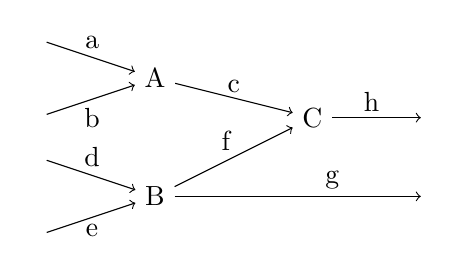
\begin{tikzpicture}
      [scale=.5, auto=center]
      \node (a) at (0,5) {};
      \node (b) at (0,3) {};
      \node (d) at (0,2) {};
      \node (e) at (0,0) {};
      \node (h) at (10,3) {};
      \node (A) at (3,4) {A};
      \node (B) at (3,1) {B};
      \node (C) at (7,3) {C};
      \node (g) at (10,1) {};
      \node (a_1) at (1.4,4.9) {a};
      \node (b_1) at (1.4,3) {b};
      \node (d_1) at (1.4,2) {d};
      \node (e_1) at (1.4,0.14) {e};
      \node (c_1) at (5,3.8) {c};
      \node (f_1) at (4.8,2.4) {f};
      \node (g_1) at (7.5,1.4) {g};
      \node (h_1) at (8.5,3.4) {h};
      \draw[->]
          (a) edge (A) (b) edge (A) (d) edge (B) (e) edge (B) (A) edge (C) (C) edge (h) (B) edge (g) (B) edge (C); 
  \end{tikzpicture}
  \end{center}
  where the "inputs" at each node are covectors and the "outputs" are vectors. Therefore, the entire diagram, which represents the tensor $X$ has a total of 4 inputs (indices $a, b, d, e$) and two outputs (indices $h, g$). We can see from the diagram that the indices $c$ and $f$, which travels "between" the factors are the ones that are being contracted. Therefore, the contraction of $c$ and $f$ contracts the rank (4,6) tensor $A \otimes B \otimes C$ to a rank (2,4) tensor. 
  \end{definition}

  \begin{definition}
  The \textbf{tensor algebra} of vector space $V$ over field $\mathbb{F}$ is an associative, noncommutative algebra defined
  \begin{align*}
      T(V) \equiv \bigoplus_{n = 0}^{\infty} V^{\otimes n} & = V^{\otimes 0} \oplus V^{\otimes 1} \oplus V^{\otimes 2} \oplus V^{\otimes 3} \oplus ... \\
      & = \mathbb{F} \oplus V \oplus V^{\otimes 2} \oplus V^{\otimes 3} \oplus V^{\otimes 4} \oplus ...
  \end{align*}
  with elements being infinite-tuples
  \[ (a, B^\mu, C^{\nu \gamma}, D^{\alpha \beta \epsilon}, ...)\]
  The addition operation is defined component-wise, and the multiplication operation is the tensor product 
  \[\otimes: T(V) \times T(V) \longrightarrow T(V)\]
  and the identity element is
  \[I = (1, 0, 0, ...) \]
  Linearity is easily proved. 
  \end{definition}

  The tensor algebra is used to "add" differently ranked tensors together. In order to do this rigorously, we must define the map (which is also an isomorphism)
  \[i_j: V^{\otimes j} \longrightarrow T(V), \; i_j (T^{\kappa_1, ..., \kappa j}) = (0, ...,0, T^{\kappa_1, ..., \kappa j}, 0, ..., 0) \]
  So, we can implicitly define the addition of arbitrary tensors $A \in V^{\otimes n}$ and $B \in V^{\otimes m}$ as 
  \[ A + B \equiv i_n (A) + i_m (B) \in T(V)\]
  along with the tensor multiplication of the form
  \[ A \otimes B \equiv i_n(A) \otimes i_m(B) \equiv i_{n+m} (A \otimes B)\]
  This allows us to alternatively define the tensor product operation as
  \[i_i(V^{\otimes i}) \otimes i_j( V^{\otimes j}) \equiv i_{i+j} (V^{\otimes (i+j)})\]

\subsection{Exterior Algebras and Symmetric Algebras}

  We can define the symmetric and exterior algebras multiple ways. In here, we will construct their powers separately as quotient spaces and direct sum them to create their respective algebras. But first, we must introduce the Schmidt decomposition, which is the foundation of all the results of this section. 

  \begin{theorem}[Schmidt Decomposition]
  For any $w \in U \otimes V$, where $U, V$ ($\dim{U} = n, \dim{V} = m$)  are inner product spaces over $\mathbb{F} \in \{ \mathbb{R}, \mathbb{C}\}$, there exists an orthonormal basis $\{u_i\}$ of $U$ and $\{v_j\}$ of $V$ such that 
  \[ w = \sum_{i=1}^{\min{\{n, m\}}} \alpha_i u_i \otimes v_i, \; \alpha_i \in \mathbb{F}\]
  \end{theorem}
  \begin{proof}
  Since $U \otimes V \simeq $ Hom$(V^*, U)$, we can interpret $w$ as a matrix $\Tilde{w}$. Using singular value decomposition, there exists unitary matrices $A, B$ and diagonal matrix $\Sigma$ such that
  \[\Tilde{w} = A \Sigma B^\dagger\]
  $C(A)$ and $R(B^\dagger)$ determine the orthonormal basis of $U \otimes V$, and we can thus see that the minimum number of required $u \otimes v$'s is precisely the number of nonzero singular values, which is the rank of $\Tilde{w}$. 

  \end{proof}

  \begin{definition}
  Let $I$ be a subspace of $V \otimes V$ generated by elements of the form $x \otimes x \in V \otimes V$. That is, given a basis $\{e_i\}$ of $n$-dimensional space $V$, all tensors of the form $x \otimes x \in V \otimes V$ can be written 
  \[x \otimes x = \sum_{i=1}^n a_i (e_i \otimes e_i) + \sum_{i \neq j} b_{i j} (e_i \otimes e_j + e_j \otimes e_i)\]
  which implies that the components of $e_i \otimes e_j$ and $e_j \otimes e_i$ must be the same for every element in $I$. 
  \end{definition}

  \begin{example}
  Given that $V$ is 2-dimensional, a vector $x \in V$ can be written $x = a e_1 + b e_2$, which implies
  \begin{align*}
      x \otimes x & = (a e_1 + b e_2) \otimes (a e_1 + b e_2) \\
      & = a^2 (e_1 \otimes e_1) + a b (e_1 \otimes e_2) + b a (e_2 \otimes e_1) + b^2 (e_2 \otimes e_2) \\
      & = a^2 (e_1 \otimes e_1) + b^2 (e_2 \otimes e_2) + a b (e_1 \otimes e_2 + e_2 \otimes e_1) 
  \end{align*}
  \end{example}

  Since we can group the components $e_i \otimes e_j$ and $e_j \otimes e_i$ together to $e_i \otimes e_j + e_j \otimes e_i$, the basis of $I$ is 
  \[\{e_1 \otimes e_1, ..., e_n \otimes e_n, e_1 \otimes e_2 + e_2 \otimes e_1, ..., e_{n-1} \otimes e_n + e_n \otimes e_{n-1}\}\]

  \begin{definition}
  Now, we can define the \textbf{second exterior power of $V$} as
  \[\Lambda^2 V \equiv \frac{V \otimes V}{I}\]
  and it follows that 
  \[\dim{\Lambda^2 V} = n^2 - \dim{I} = \frac{1}{2} n (n-1)\]
  We denote the elements of $\Lambda^2 V$ as $x \wedge y$, which really just represents the equivalence class of $x \otimes y$ in the quotient space. It is clear that $x \otimes x \in I \implies x \wedge x = 0$, so
  \begin{align*}
      0 = (x + y) \wedge (x + y) & = x \wedge x + x \wedge y + y \wedge x + y \wedge y \\
      & = x \wedge y + y \wedge x \\
      \implies & x \wedge y = - y \wedge x
  \end{align*}
  That is, the wedge product is antisymmetric. Note also that we can assume distributivity of $\wedge$ since it is just the quotient operation of another operation $\otimes$ that satisfies distributivity. We can construct a basis on $\Lambda^2 V$, given by 
  \[\{e_i \wedge e_j \; | \; i < j\}\]
  Again, we note that $i < j$ since $e_i \wedge e_i = 0$ and $e_i \wedge e_j = - e_j \wedge e_i$. 
  \end{definition}

  One realization of the space $\Lambda^2 \mathbb{R}^n$ is the set of antisymmetric $n \times n$ matrices. We can construct higher order exterior powers, too. For $n = 3$ (and assuming that $\dim{V} \geq 3$), the subspace $I \subset V \otimes V \otimes V$ is the space generated by elements of the forms
  \[x \otimes x \otimes y, x \otimes y \otimes x, y \otimes x \otimes x\]
  Following a similar construction, the \textbf{third exterior power of $V$} is
  \[\Lambda^3 V \equiv \frac{V \otimes V \otimes V}{I}\]
  with its elements being equivalence classes of the form
  \[x \wedge y \wedge z,\; x, y, z \in V\]
  such that
  \begin{align*}
      x \wedge y \wedge z & = - x \wedge z \wedge y \\
      & = - y \wedge x \wedge z \\
      & = - z \wedge y \wedge x
  \end{align*}
  The basis of $\Lambda^3 V$ is
  \[\{e_i \wedge e_j \wedge e_k \; | \; i < j < k\} \implies \dim{\Lambda^3 V} = \frac{1}{6} n (n-1) (n-2)\]
  Generally, if $\sigma$ is a permutation of the ordered list $(1, 2, ..., n)$, and $x_1, x_2, ..., x_n \in V$, then 
  \[x_{\sigma(1)} \wedge x_{\sigma(2)} \wedge ... \wedge_{\sigma(n)} = sgn(\sigma) \; x_1 \wedge x_2 \wedge ... \wedge x_n\]
  which means that if $x_i = x_j$ for some $1 \leq i \neq j \leq n$, 
  \[x_1 \wedge x_2 \wedge ... \wedge x_n = 0\]
  By constructing all the exterior powers of $n$-dimensional space $V$, we can construct the algebra 
  \begin{align*}
      \Lambda(V) \equiv \bigoplus_{k=0}^n \Lambda^k V \equiv \Lambda^0 V \oplus \Lambda^1 V \oplus \Lambda^2 V \oplus ... \oplus \Lambda^n V 
  \end{align*}
  Note that $\Lambda^0 V = \mathbb{F}$ and $\Lambda^1 V = V$. Unlike the tensor algebra, the exterior algebra is finite since the exterior powers vanish for finite $n$. In fact, 
  \[ \dim{\Lambda^k V} = \begin{cases}
  _n C_k & 0 \leq k \leq n \\
  0 & n < k
  \end{cases}\]
  which implies that 
  \[\dim{\Lambda(V)} = 2^n \]
  \begin{definition}
  The $n$th exterior power $\Lambda^n V$ is 1 dimensional, spanned by the singular basis vector 
  \[e_1 \wedge e_2 \wedge ... \wedge e_{n-1} \wedge e_n\]
  This vector is the \textit{determinant}. Note that this construction of the determinant is consistent with our previous construction of the determinant of a matrix since $e_1 \wedge ... \wedge e_n$ is indeed multilinear and antisymmetric. In its purest sense, 
  \[e_1 \wedge ... \wedge e_n: \prod_{i=1}^n V^* \longrightarrow \mathbb{F}\]
  is a mapping that is multilinear and antisymmetric. But there is an inconsistency. The matrix determinant takes in \textit{matrices} rather than taking in $n$-tuples of covectors. However, we can interpret the $n$ covectors in $V^* \times ... \times V^*$ as the column (or row) vectors of an $n \times n$ matrix. This completes the realization, and so we can conclude that the matrix determinant is just a realization of the more abstract determinant $e_1 \wedge ... \wedge e_n$. 

  Note that any tensor in $\Lambda^n V$ satisfies multilinearity and antisymmetricity, but only the basis vector $e_1 \wedge ... \wedge e_n$ satisfies the normalizing condition
  \[\det{I} = 1\]
  Since, given that the dual basis of $V^*$ is $\{f_j\}$
  \[(e_1 \wedge ... \wedge e_n) (f_1, f_2, ..., f_n) = \prod_{i=1}^n e_i (f_i) = \prod_{i=1}^n \delta_i^i = 1\]
  \end{definition}

  \begin{example}
  Given 3 dimensional vector space $V$ with basis $\{e_1, e_2, e_3\}$, the wedge product of two vectors $a, b \in V$ is 
  \begin{align*}
      a \wedge b & = (a_1 e_1 + a_2 e_2 + a_3 e_3) \wedge (b_1 e_1 + b_2 e_2 + b_3 e_3) \\
      & = (a_2 b_3 - a_3 b_2) e_2 \wedge e_3 + (a_3 b_1 - a_1 b_3) e_3 \wedge e_1 + (a_1 b_2 - a_2 b_1) e_1 \wedge e_2 
  \end{align*}
  which is essentially the formula for the cross product $\times$ in Euclidean space. We can therefore think of the realization of the wedge product in 3 dimensional space $V$ as the cross product. 
  \[\wedge: V \times V \longrightarrow \Lambda^2 V\]
  Note that $\Lambda^2 V \simeq V$ if $\dim{V} = 3$, so we can construct the more familiar $\times$ operation in $\mathbb{R}^3$. 
  \[\times: \mathbb{R}^3 \times \mathbb{R}^3 \longrightarrow \Lambda^2 \mathbb{R}^3 \simeq \mathbb{R}^3\]
  which is consistent with $\times$ taking two vectors and outputting a third vector living in $\mathbb{R}^3$ that is orthogonal to the two input vectors. 
  \end{example}

  \begin{example}
  The realization of the wedge product of 3 vectors in 3 dimensional space $V$ is the \textit{triple scalar product}, which we will denote as $\times_3$
  \[\wedge: V \times V \times V \longrightarrow \Lambda^3 V\]
  Note that since $\Lambda^3 V \simeq V$ when $\dim{V} = 3$, we can write 
  \[\times_3: \mathbb{R}^3 \times \mathbb{R}^3 \times \mathbb{R}^3 \longrightarrow \Lambda^3 \mathbb{R}^3 \simeq \mathbb{R}\]
  which is consistent with $\times_3$ taking three vectors and outputting the signed volume of their parallelopiped which lies in $\mathbb{R}$. 
  \end{example}

  Now we introduce the symmetric algebra and its construction. Let $I$ be the subspace of $V \otimes V$ generated by all tensors of the form 
  \[u \otimes v - v \otimes u, \; u, v \in V\]
  For example, given $a, b \in V$ with basis $\{e_1, e_2\}$, 
  \begin{align*}
      a \otimes b - b \otimes a & = (a_1 e_1 + a_2 e_2) \otimes (b_1 e_1 + b_2 e_2) - (b_1 e_1 + b_2 e_2) \otimes (a_1 e_1 + a_2 e_2) \\
      & = (a_1 b_2 - b_2 a_1) e_1 \otimes e_2 + (a_2 b_1 - b_2 a_1) e_2 \otimes e_1 
  \end{align*}
  is an element of $I$. We can generalize this to see that
  \[\{e_i \otimes e_j - e_j \otimes e_i\}, \; i \neq j\]
  is the basis for $I$. Now, let us define the \textit{second symmetric power of $V$} as 
  \[\Sym^2 V \equiv \frac{V \otimes V}{I}\]
  where, given that $\dim{V} = n$, 
  \[\dim{\Sym^2 V} = n^2 - \frac{1}{2} n (n-1) = \frac{1}{2} n (n+1)\]
  We denote the elements of $\Sym^2 V$ as $x \odot y$, which are really the equivalence classes $\{x \otimes y - y \otimes x\}$. Note that
  \begin{align*}
      x \odot y - y \odot x & = \{x \otimes y - y \otimes x\} - \{ y \otimes x - x \otimes y\} \\
      & = \{ x \otimes y - y \otimes x - y \otimes x + x \otimes y\} \\
      & = \{0\} = 0
  \end{align*}
  $\implies x \odot y = y \odot x$. That is, the $\odot$ operator is symmetric, and $\Sym^2 V$ has basis 
  \[ \{e_i \odot e_j\}_{j \geq k}\]
  One realization of $\Sym^2 \mathbb{R}^n$ is the set of all symmetric $n \times n$ real matrices. We can construct higher symmetric powers satisfying this property that its tensors are invariant under transpositions. 
  \[x_1 \odot ... x_i \odot ... x_j \odot ... x_n = x_1 \odot ... x_j \odot ... x_i \odot ... x_n\]
  for all $1 \leq i \neq j \leq n$, which implies that it is invariant under any permutation $p \in S_n$ of the $x_i$'s. Additionally, 
  \[\dim{\Sym^k V} = \binom{n+k-1}{k}\]

  \begin{definition}
  The \textbf{symmetric algebra} of vector space $V$ is constructed as such 
  \[\Sym (V) \equiv \bigoplus_{k=0}^\infty \Sym^k V\]
  Note that unlike the exterior algebra, $\Sym(V)$ is infinite dimensional. 
  \end{definition}

  \begin{example}
  The inner product $(\cdot, \cdot)$ on $V$ is an element of $\Sym^2 V$, since it is a bilinear, symmetric operation on $V$. 
  \[\odot, (\cdot, \cdot): V \times V \longrightarrow \mathbb{F}\]
  \end{example}

  There is a simple relationship between $V \otimes V$, $\Lambda^2 V$, and $\Sym^2 V$. 

  \begin{theorem}
  \[V \otimes V \simeq \Sym^2 V \oplus \Lambda^2 V\]
  with isomorphism defined
  \[v \otimes w \mapsto \Big( \frac{1}{2} (v \odot w), \frac{1}{2} (v \wedge w) \Big)\]
  This is precisely the factoring of a rank (2,0) tensor into its symmetric and antisymmetric parts. 
  \end{theorem}
  \begin{proof}
  Given $v \otimes w \in V \otimes V$, 
  \[v \otimes w + w \otimes v \in \Sym^2 V \text{ and } v \otimes w - w \otimes v \in \Lambda^2 V\]
  By defining $v \odot w$ and $v \wedge w$ as the expressions above, the isomorphism is satisfied. 
  \end{proof}

  Therefore, when working in $V \otimes V$, we can interpret 
  \begin{align*}
      & v \wedge w = \frac{1}{2} (v \otimes w - w \otimes v) \\
      & v \odot w = \frac{1}{2} (v \otimes w + w \otimes v) 
  \end{align*}

  However, 
  \[V \otimes V \otimes V \not\simeq \Sym^3 V \oplus \Lambda^3 V\]
  \textit{Schur functors} are used to fix this discrepancy. 

  Note that we have introduced these two algebras by first constructing the quotient spaces $\Lambda^n V$ and $\Sym ^n V$ from the tensor product spaces $T^{\otimes n}$ and then direct summing these powers to construct the algebras. We will introduce another type of construction that directly takes the quotient algebra of $T(V)$ with the two-sided ideal. 

